\appendix
\section{Circuit Design}
\subsection*{Wave Generator}
\begin{figure}[h]
    \centering
    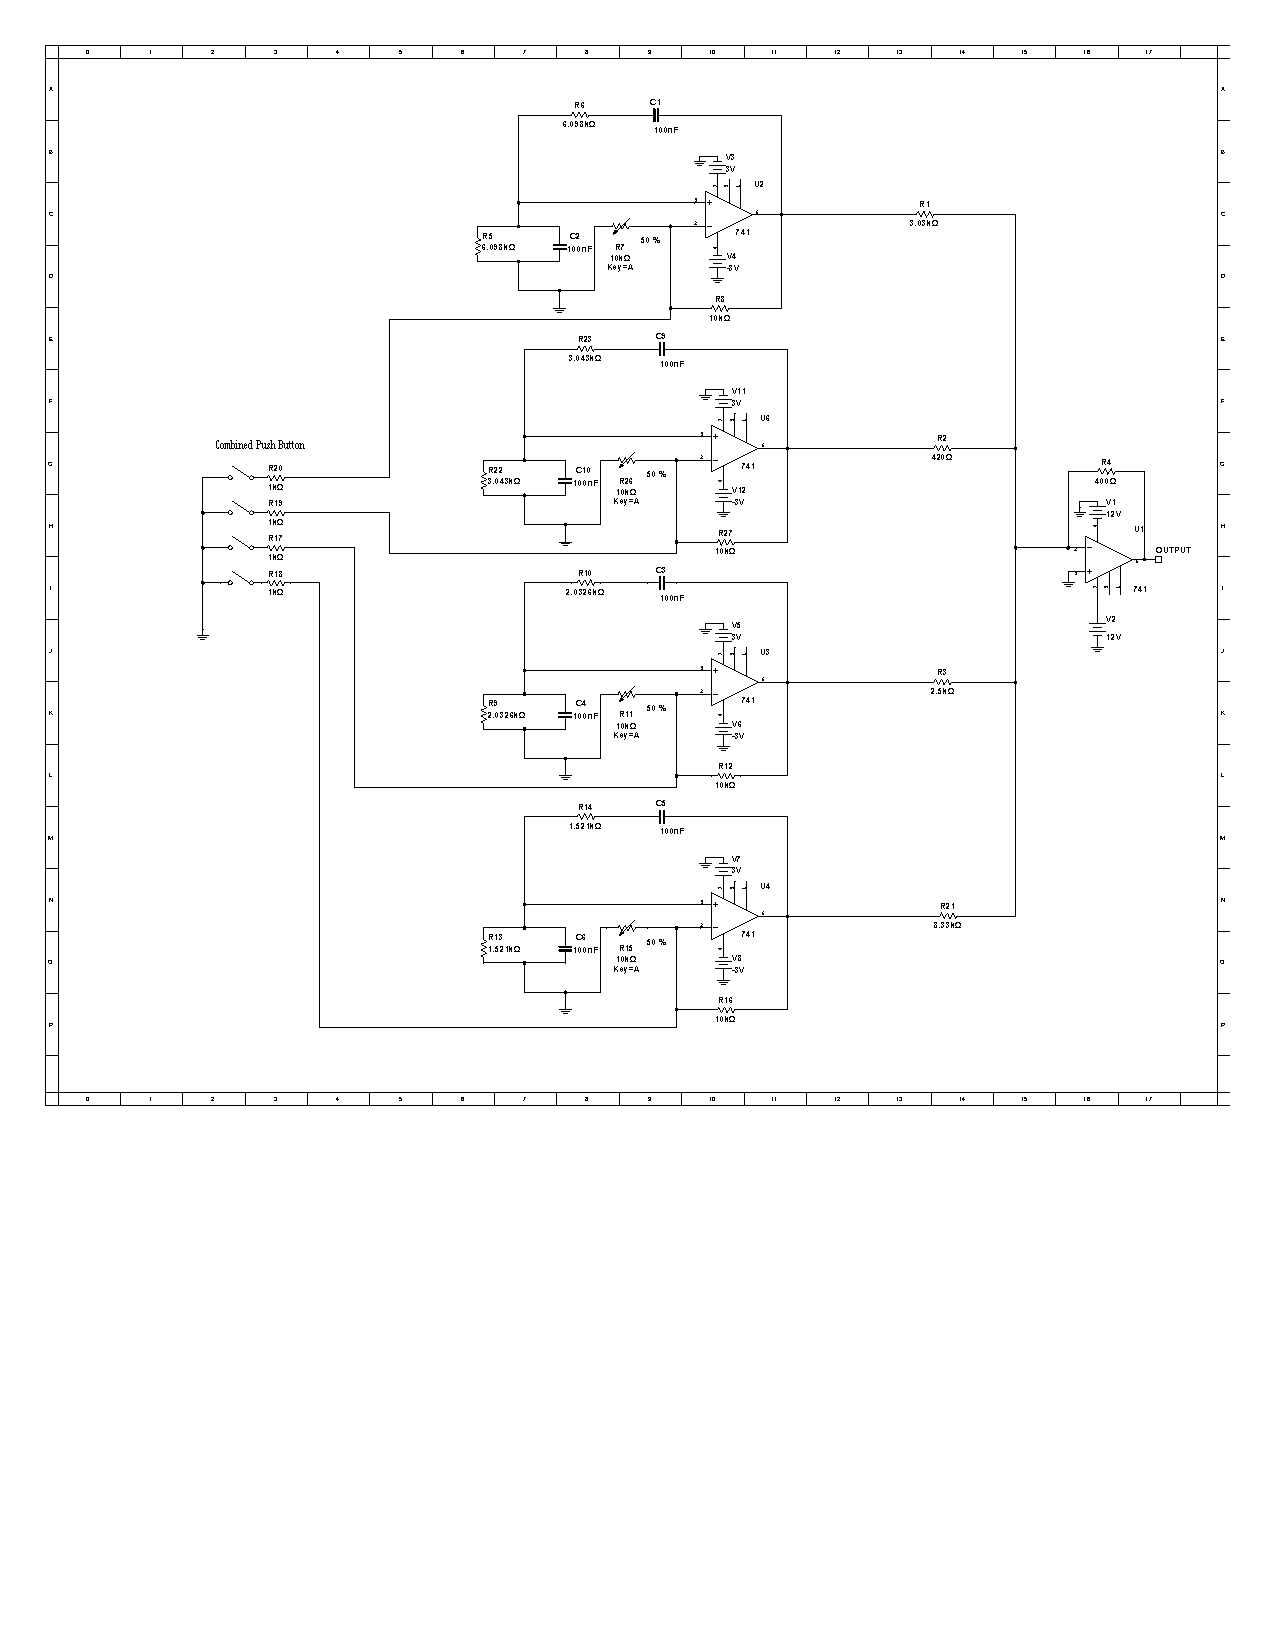
\includegraphics[width=.65\textwidth]{oscillator_mul}
    \vspace*{-5cm}
\end{figure}
\subsection*{Amplifier}
\begin{figure}
    \centering
    \vspace*{-6.5cm}
    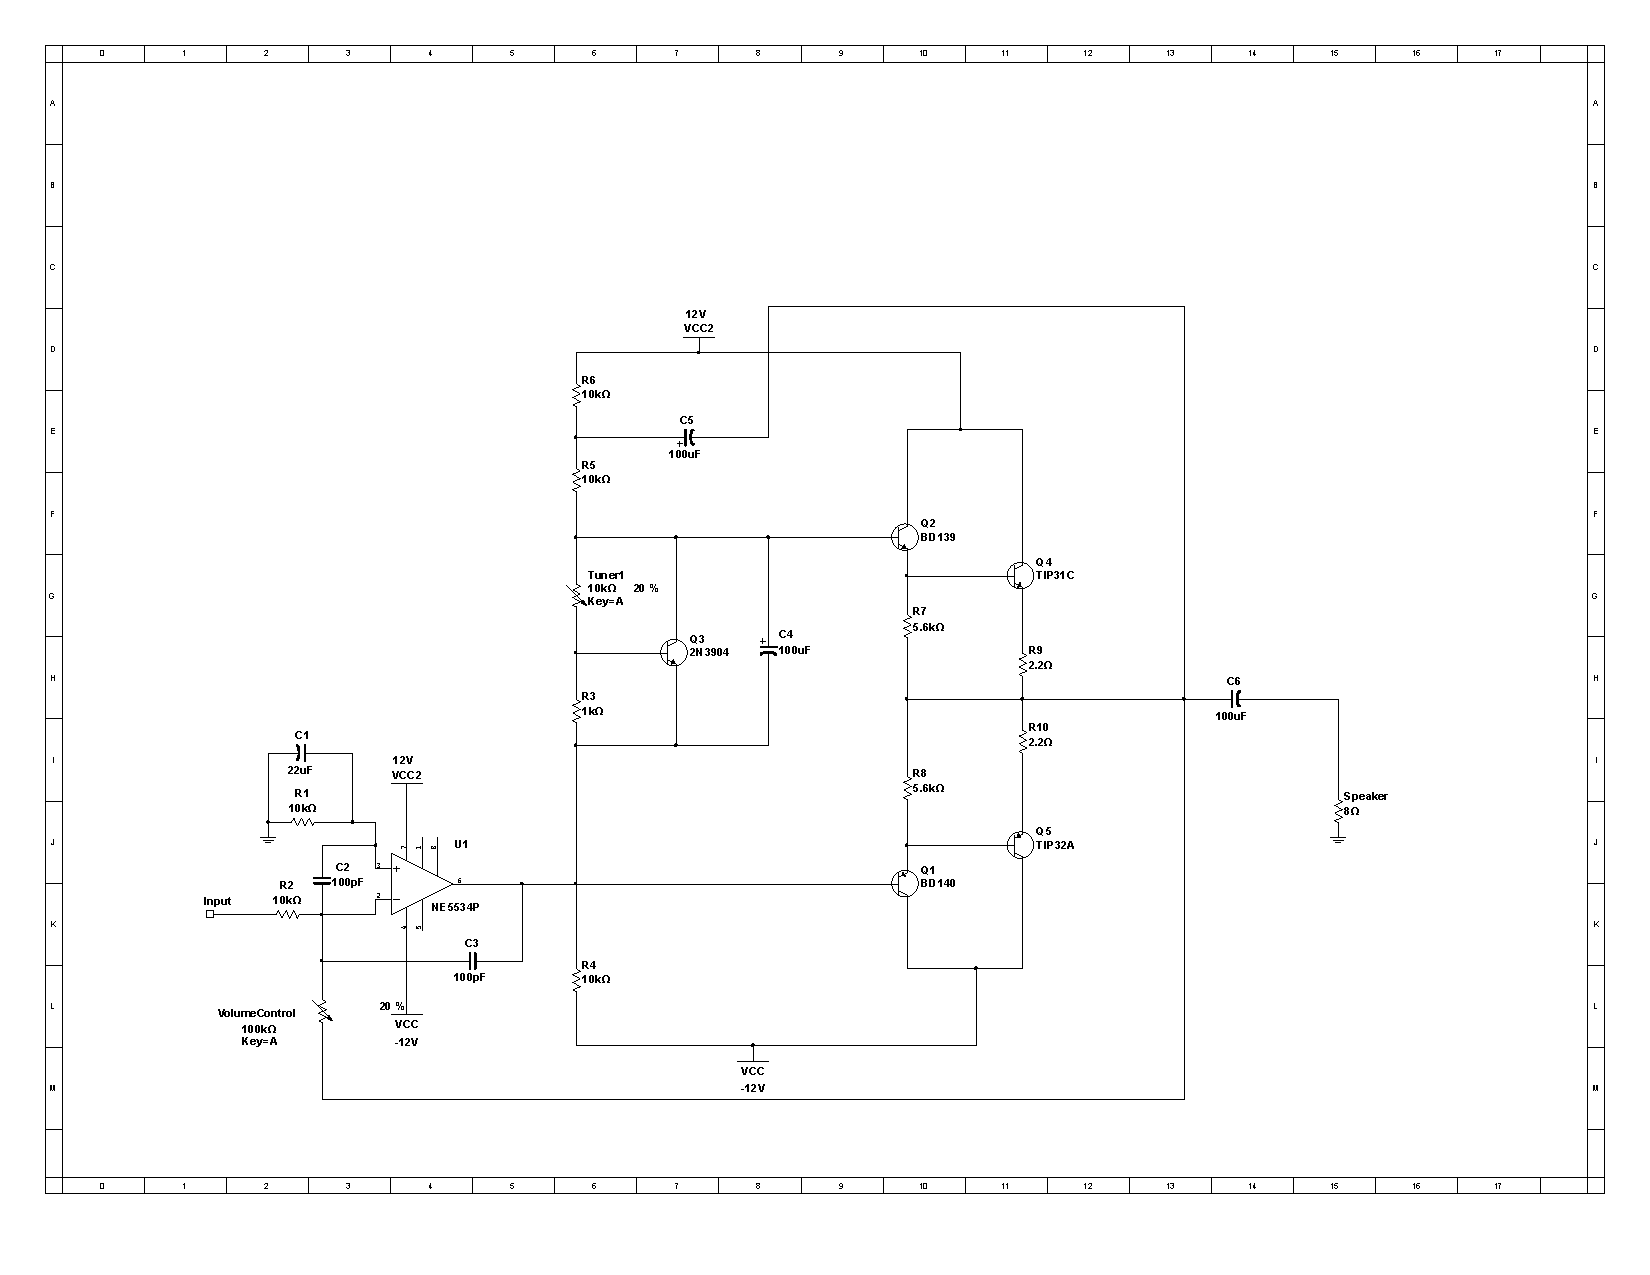
\includegraphics[width=.85\textwidth]{amplifier_mul}
\end{figure}
\newpage

\section{Layout}
\begin{figure}[h]
    
    \begin{subfigure}{\textwidth}
        \centering
        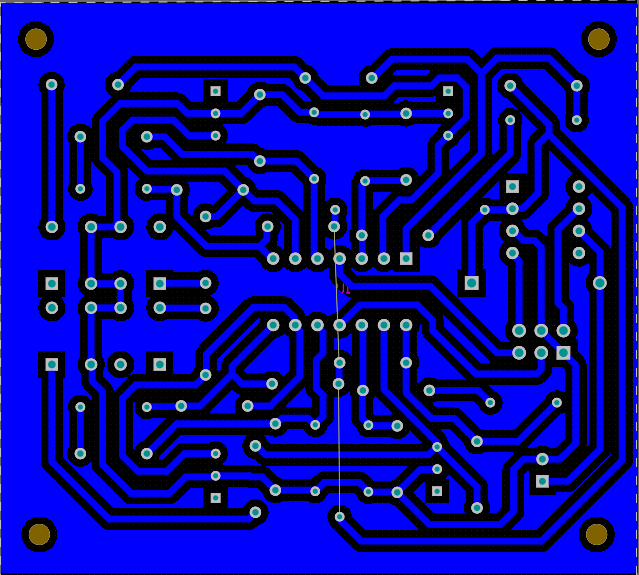
\includegraphics[width=.55\textwidth]{osc_lay}
        \caption{\textbf{PCB-I} : Wave Generator}
    \end{subfigure}
    \vspace*{.5cm}
    \begin{subfigure}{\textwidth}
        \centering
        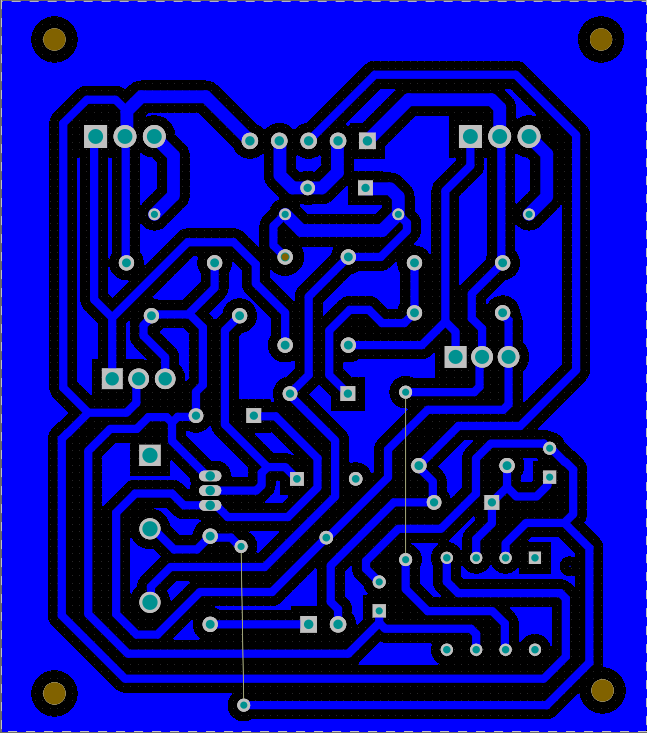
\includegraphics[width=.45\textwidth]{amp_lay}
        \caption{\textbf{PCB-II} : Amplifier}
    \end{subfigure}
\end{figure}
\section{Datasheet}
The datasheet of the model is as follows...
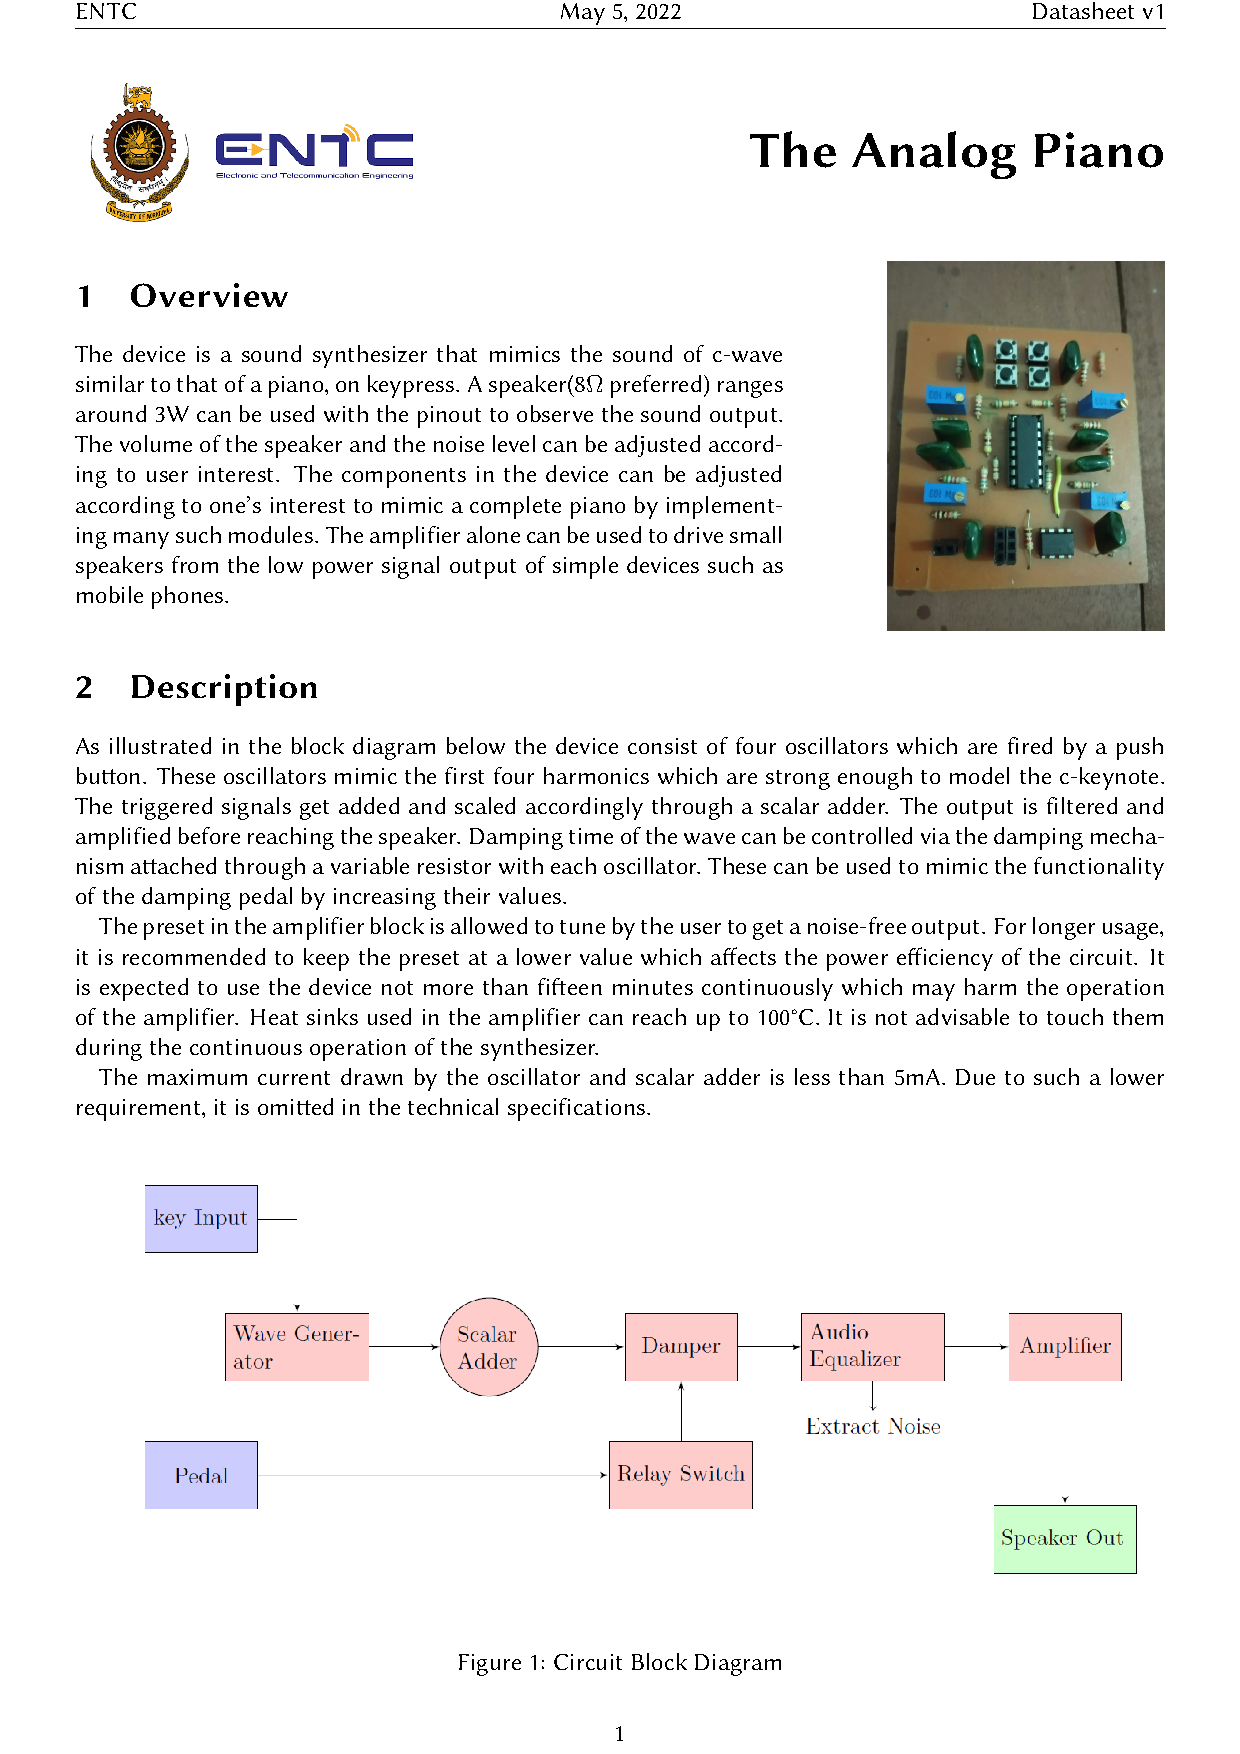
\includepdf[pages=-]{sections/datasheet}